\chapter{Registrador de status (\texttt{reg\_status})}
\label{cap:reg_status}

\section{Especificação}

O \texttt{reg\_status} tem cinco registradores independentes de 1 bit, chamados RN, RV, RZ, RH e RC, que guardam as \textit{flags} produzidas pela ALU do TP1 (negativo, \textit{overflow}, zero, \textit{half carry/borrow} e \textit{carry/borrow}) \cite{tp2}. Entradas, saídas e habilitações são vetores de 5 bits, e cada bit corresponde a um registrador. Um registrador só é escrito, na borda de subida do clock, se a sua habilitação individual estiver ativa. O reset assíncrono zera os cinco e tem preferência sobre as demais entradas. A saída é sempre ativa e não depende do clock nem de habilitação. A Figura~\ref{fig:bloco-reg-status} mostra o diagrama de blocos e o Quadro~\ref{quad:portas-reg-status} descreve as portas.

\begin{figure}[htb]
\caption{Diagrama de blocos do registrador de status.}\label{fig:bloco-reg-status}
\centering
\begin{tikzpicture}[>={Stealth[length=2mm]}]
  \renewcommand{\fio}{0.8}
  \node[draw, minimum width=3.4cm, minimum height=3.6cm, font=\large\bfseries] (bloco) {reg\_status};
  \pentrada{1.4}{nrst}{}
  \pentrada{0.6}{clk\_in}{}
  \pentrada{-0.2}{status\_reg\_in[4..0]}{line width=1.2pt}
  \pentrada{-1.0}{status\_reg\_wr\_ena[4..0]}{line width=1.2pt}
  \psaida{0.2}{status\_reg\_out[4..0]}{line width=1.2pt}
\end{tikzpicture}
\fonte{Elaborada pelos autores, com base em \textcite{tp2}.}
\end{figure}

\begin{quadro}[htb]
  \caption{Portas do registrador de status.}
  \label{quad:portas-reg-status}
  \centering
  \begin{tabular}{lcp{7.4cm}}
    \hline
    Porta & Direção & Descrição \\ \hline
    \texttt{nrst} & entrada & \textit{Reset} assíncrono, ativo em nível baixo; zera os cinco registradores \\
    \texttt{clk\_in} & entrada & Clock; a escrita acontece na borda de subida \\
    \texttt{status\_reg\_in[4..0]} & entrada & Dados: [0] RN, [1] RV, [2] RZ, [3] RH, [4] RC \\
    \texttt{status\_reg\_wr\_ena[4..0]} & entrada & Habilitação de escrita de cada registrador, ativa em nível alto, na mesma ordem dos dados \\
    \texttt{status\_reg\_out[4..0]} & saída & Conteúdo dos cinco registradores, na mesma ordem \\ \hline
  \end{tabular}
  \fonte{Adaptado de \textcite{tp2}.}
\end{quadro}

A ordem dos bits é a mesma do vetor \texttt{flags\_out} da ALU (Quadro~\ref{qua:flags-alu}), de modo que a saída da ALU pode ser ligada diretamente à entrada do registrador de status.

\begin{quadro}[htb]
  \caption{Correspondência entre as \textit{flags} da ALU e os registradores de status.}
  \label{qua:flags-alu}
  \centering
  \begin{tabular}{cll}
    \hline
    Bit & Registrador & \textit{Flag} da ALU (\texttt{flags\_out}) \\ \hline
    0 & RN & \textit{negative} (\texttt{n\_flag}) \\
    1 & RV & \textit{overflow} (\texttt{v\_flag}) \\
    2 & RZ & \textit{zero} (\texttt{z\_flag}) \\
    3 & RH & \textit{half carry/borrow} (\texttt{h\_flag}) \\
    4 & RC & \textit{carry/borrow} (\texttt{c\_flag}) \\ \hline
  \end{tabular}
  \fonte{Adaptado de \textcite{tp2}.}
\end{quadro}

\section{Implementação}

\subsection{Arquitetura}

O bloco tem um vetor de estado de 5 bits e é descrito em duas partes:

\begin{itemize}
  \item \textbf{Próximo estado} (concorrente): cada bit do próximo estado é um multiplexador 2:1 controlado pela habilitação do próprio bit, escrito como uma expressão lógica sobre vetores, \texttt{(entrada AND ena) OR (estado AND NOT ena)}. Habilitado, o bit recebe a entrada; senão, mantém o valor atual. Como a expressão é bit a bit, os cinco registradores ficam independentes sem nenhum laço.
  \item \textbf{Registrador} (\texttt{process}): sensível a \texttt{nrst} e \texttt{clk\_in}, zera o estado com o reset e, na borda de subida, carrega o próximo estado.
\end{itemize}

A saída \texttt{status\_reg\_out} é uma atribuição concorrente do vetor de estado, e portanto não depende de clock nem de habilitação.

\subsection{Decisões de projeto}

\begin{itemize}
  \item \textbf{Habilitação fora do \texttt{process}}: com a habilitação por bit, a alternativa seria um \texttt{IF} por registrador dentro do processo, ou um laço. A expressão sobre vetores é mais curta e deixa o processo igual ao dos demais blocos (reset e carga), com a lógica de escolha à parte.
  \item \textbf{Prioridade do reset}: \texttt{nrst} é o primeiro teste do \texttt{IF}, antes da borda de subida, de modo que vale mesmo com habilitações ativas, e age independentemente do clock.
\end{itemize}

\subsection{Circuito em nível RTL}

A Figura~\ref{fig:rtl-reg-status} mostra a interpretação feita pelo RapidRTL: um único \texttt{\$adff} de 5 bits (\textit{flip-flops} com reset assíncrono), cuja entrada D vem de portas E, inversor e OU, exatamente a expressão do próximo estado. O sintetizador do Quartus aloca 5 elementos lógicos e 5 \textit{flip-flops}.

\begin{figure}[htb]
  \centering
  \caption{Circuito do registrador de status em nível RTL.}
  \label{fig:rtl-reg-status}
  \includegraphics[width=0.9\textwidth, height=0.4\textheight, keepaspectratio]{reg_status_rtl.pdf}
  \fonte{Elaborado a partir do site RapidRTL, com base no arquivo \texttt{project/reg\_status/reg\_status.vhd}.}
\end{figure}

\subsection{Código-fonte}

O Código~\ref{lst:reg-status} apresenta a entidade e a arquitetura completas, com comentários.

\blocovhdl{Descrição VHDL do registrador de status.}{lst:reg-status}{reg_status}{reg_status.vhd}

\section{Simulação e resultados}

\subsection{Metodologia}

O projeto tem cinco formas de onda (arquivos \texttt{.vwf} em \texttt{project/reg\_status/}), todas com clock de 20\,ns e reset inicial:

\begin{itemize}
  \item \texttt{reg\_status.vwf}: visão geral, com escrita de todos os bits, zeragem um bit por vez e escrita parcial;
  \item \texttt{reg\_status\_escrita.vwf}: escrita de todos os bits com padrões alternados;
  \item \texttt{reg\_status\_enable.vwf}: uma habilitação por vez, setando e zerando cada registrador, e dados diferentes dos armazenados;
  \item \texttt{reg\_status\_alu.vwf}: uso real, simulando o armazenamento das \textit{flags} de ADD, AND, SUB, XOR e SRA da ALU, e atualizando só as \textit{flags} que cada operação define;
  \item \texttt{reg\_status\_reset.vwf}: reset fora de qualquer borda, reset prevalecendo sobre a escrita e pulso curto de reset.
\end{itemize}

O \textit{testbench} \texttt{extras/reg\_status\_tb.vhd} compara a saída com um modelo bit a bit, em casos direcionados e em 500 ciclos pseudoaleatórios de dados e habilitações; são 517 comparações, sem nenhuma falha. As tabelas de resultados esperados estão em \texttt{extras/casos\_de\_teste.md}.

\subsection{Casos de teste e resultados}

A Figura~\ref{fig:sim-reg-status} mostra a simulação de \texttt{reg\_status.vwf} e a Tabela~\ref{tab:caso-reg-status} traz os valores esperados. Cada linha é um intervalo entre mudanças das entradas, com as saídas do fim do intervalo. As tabelas das demais formas de onda estão no Apêndice~\ref{ap:tabelas}.

\begin{figure}[htb]
  \centering
  \caption{Simulação funcional de \texttt{reg\_status.vwf} (visão geral).}
  \label{fig:sim-reg-status}
  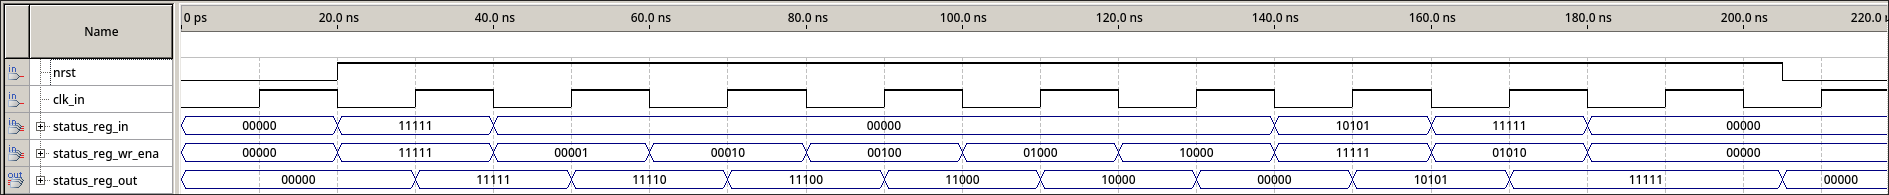
\includegraphics[width=\textwidth]{../../project/reg_status/reg_status_simulation.png}
  \fonte{Autoria própria (Quartus II).}
\end{figure}

\Needspace*{12\baselineskip}
{\scriptsize\setlength{\tabcolsep}{3pt}
\begin{longtable}{rccccp{4.4cm}}
\caption{Casos de teste de \texttt{reg\_status.vwf}: visão geral.}
\label{tab:caso-reg-status}\\
\hline $t$ (ns) & \texttt{nrst} & \texttt{status\_reg\_in} & \texttt{status\_reg\_wr\_ena} & \texttt{status\_reg\_out} & Observação \\ \hline \endfirsthead
\hline $t$ (ns) & \texttt{nrst} & \texttt{status\_reg\_in} & \texttt{status\_reg\_wr\_ena} & \texttt{status\_reg\_out} & Observação \\ \hline \endhead
0--20 & 0 & 00000 & 00000 & 00000 &  \\
20--40 & 1 & 11111 & 11111 & 11111 & solta o reset; escreve 11111 (todos habilitados) \\
40--60 & 1 & 00000 & 00001 & 11110 & zera só RN \\
60--80 & 1 & 00000 & 00010 & 11100 & zera só RV \\
80--100 & 1 & 00000 & 00100 & 11000 & zera só RZ \\
100--120 & 1 & 00000 & 01000 & 10000 & zera só RH \\
120--140 & 1 & 00000 & 10000 & 00000 & zera só RC \\
140--160 & 1 & 10101 & 11111 & 10101 & escreve 10101 em todos \\
160--180 & 1 & 11111 & 01010 & 11111 & in = 11111, mas só RV e RH habilitados \\
180--205 & 1 & 00000 & 00000 & 11111 & ninguém habilitado: mantém \\
205--220 & 0 & 00000 & 00000 & 00000 & reset assíncrono \\
\hline
\end{longtable}}
\vspace{-0.9cm}
\fonte{Autoria própria. Saídas do fim de cada intervalo, conforme o modelo de referência e a simulação do Quartus II.}


\subsection{Análise dos resultados}

\begin{itemize}
  \item \textbf{Escrita total}: com as cinco habilitações ativas, a escrita de \texttt{11111} na borda de 30\,ns leva a saída de \texttt{00000} a \texttt{11111}.
  \item \textbf{Habilitação individual}: de 40 a 140\,ns, \texttt{status\_reg\_in} fica em \texttt{00000} e uma habilitação é ativada por vez (\texttt{00001}, \texttt{00010}, \texttt{00100}, \texttt{01000}, \texttt{10000}). A saída passa por \texttt{11110}, \texttt{11100}, \texttt{11000}, \texttt{10000} e \texttt{00000}: só o registrador habilitado é zerado, e os demais mantêm o valor.
  \item \textbf{Escrita parcial}: com \texttt{status\_reg\_in = 11111} e habilitação \texttt{01010}, apenas RV e RH recebem 1, e a saída passa de \texttt{10101} para \texttt{11111}, pois os outros três bits já valiam 1 e continuam como estavam. O papel de cada entrada fica mais evidente em \texttt{reg\_status\_enable.vwf}, em que o dado e a habilitação são diferentes entre si.
  \item \textbf{Sem habilitação}: em 180--200\,ns, com \texttt{status\_reg\_wr\_ena = 00000}, o clock continua mudando e a saída não se altera.
  \item \textbf{Reset assíncrono}: em 205\,ns, no meio do ciclo, \texttt{nrst} cai e a saída vai a \texttt{00000} na hora.
\end{itemize}

A forma de onda \texttt{reg\_status\_alu.vwf} mostra o uso pretendido: depois de uma soma que atualiza as cinco \textit{flags}, uma operação lógica atualiza só N e Z (habilitação \texttt{00101}), e as \textit{flags} C, H e V, que a ALU deixa indefinidas nessas operações, preservam o valor anterior.
